\documentclass[10pt,a4paper]{article}
\usepackage[utf8]{inputenc}
\usepackage[T1]{fontenc}
\usepackage{lmodern}
\usepackage[margin=2.2cm]{geometry}
\usepackage{graphicx}
\usepackage{booktabs}
\usepackage{microtype}
\usepackage[hidelinks]{hyperref}
\usepackage{url}

\title{Beliefs in a Meme War: Belief and Stance Mapping of the France vs Japan Clash on X After the October 17, 2026 Riots}
\author{Louis Korczowski\\
\small STATUR viral marketing lab, Cairn-Crea SASU, France\\
\small \texttt{louis@cairn-crea.com}}
\date{Preprint v1, October 29, 2026}

\begin{document}
\maketitle

\begin{abstract}
After the October 17, 2026 protests in France ended in looting, a cosplay image and a One Piece flag at the riots set off a mass exchange between French-speaking and Japanese-speaking accounts on X. We read the 327 most viewed posts of the clash (356 million views, eight language communities) and tagged each one with the belief it carries, its stance toward that belief (supports, attacks, neutral), its camp, its language community and its register (humor, argument, information, testimony, insult, meta). Eighteen beliefs account for the conflict. Four results stand out. (1) On the Japanese side, 40\% of views (51M) went to four beliefs about immigration and media distrust, led by ``It's a Muslim invasion'' (31M). (2) Official arrest data, posted by a well-known Japanese internet entrepreneur, out-reached every one of the five replies that defended the invasion belief, yet posts supporting that belief reached 8.7 times more views. (3) The French side answered the racism accusation mostly with stereotypes: three stereotype beliefs took 49\% of French-side views, against 2\% for posts accusing Japan of racism. (4) A Japanese plea to keep manga out of the riots lost 11 of 12 direct duels to French mockery. Accounts writing in neither French nor Japanese drew 23\% of views. Humor made 39\% of posts and 54\% of views. Finally, we test whether beliefs can be recovered automatically. Clustering sentence embeddings recovers little of the hand labels (adjusted Rand index 0.10 on raw multilingual posts, 0.19 on written paraphrases), and zero-shot assignment to the 18 belief labels reaches 21\% top-1 accuracy on raw text against 33\% on paraphrases (chance 6\%). Most of the gap lies in resolving what a joke implies, a step that sentence encoders do not perform. We release the belief map, per-post annotations (paraphrased, no post text) and code.
\end{abstract}

\noindent\textbf{Keywords:} social media, X (Twitter), memes, virality, stance detection, concept induction, sentence embeddings, zero-shot classification, LLM-assisted annotation, immigration discourse, France, Japan.

\section{Introduction}
Studies of online virality usually count content: posts, hashtags, formats. A meme war shows the limit of this approach. The same belief can travel as a joke, a statistic, a testimony or an insult, and a debunk spreads the belief it attacks. Counting formats hides what each side believed and which beliefs won attention.

We propose a simple unit of analysis for attention conflicts: the \emph{belief}, a claim a person could state as ``I believe that \ldots'', independent of the packaging that carries it. Each post is tagged with one belief and a stance toward it. Reach is then measured per belief and per stance, and replies that quote another post are scored as duels.

The paper makes three contributions: (1) a belief and stance annotation scheme for meme conflicts, with a four-question test for belief labels; (2) a measurement of the France vs Japan clash on X with this scheme; (3) a test of how far off-the-shelf sentence encoders can recover the beliefs, from raw multilingual posts and from written paraphrases.

We apply this to the clash between French-speaking and Japanese-speaking accounts on X that followed the October 17, 2026 protests in France. The case is useful because it mixes humor, national stereotypes, immigration discourse and a factual correction, all within ten days, with X's automatic translation putting each side's posts in front of the other.

\section{Context}
On October 17, 2026, between 550,000 (Interior Ministry) and 800,000 (organizers) people marched across France for education funding and purchasing power~\cite{franceinfo,wiki}. The evening ended in looting in Paris, Lyon, Marseille and other cities~\cite{wiki}. From October 18, images of rioters in anime cosplay and with the One Piece pirate flag circulated on X, and Japanese-speaking accounts asked the French not to involve Japanese culture. French-speaking accounts answered with jokes about Japan, and the exchange grew over the following week. On October 22, a note from the French Justice Ministry reported that, of 186 people jailed between October 18 and 21, 70\% were French nationals, nearly all of them born in France, 68\% were aged 25 or under and 95\% were men~\cite{france24}. In Japan, the debate ran alongside domestic discussion of immigration: permanent residency guidelines were revised on October 1, 2026~\cite{nippon}, and the Sanseito party, which campaigns on ``Japanese First'', had won 14 seats in the July 2025 upper house election~\cite{mashable}. Press coverage in late October described the clash without measuring it~\cite{mashable,vingt}.

\section{Data}
The corpus combines three sources: (a) 59 seed posts, every tracked post above 500,000 views plus posts collected by hand from X search; (b) 146 posts from searches by language at view thresholds of 500,000 and 250,000, plus a Japanese-language pass down to 100,000; (c) 115 quote posts read in the Quotes tab of the 15 most viewed posts, sorted by views. Posts quoted by seeds were added through the X API. After relevance vetting, the corpus holds 327 posts with 356.5 million views. Most posts date from October 18 to 26, 2026; a few quoted posts are older (earliest October 6). Post metadata came from the X API v2 (post lookup and counts), at a total API cost under 5 USD; search result pages and quote pages were read in a logged-in browser.

Daily post volume confirms the event: on the final search queries, French-language volume was 3.4 to 6.5 times its September baseline (1,734 posts per day) from October 20 to 25, and Japanese-language volume 4.8 to 9.3 times its baseline (1,565 posts per day) from October 20 to 26.

\section{Method}
\subsection{Reading and annotation}
Each post was read with its image or video, because the meaning of a meme often lives in the image~\cite{memecap}. A contact sheet of all thumbnails was inspected. Each post received: an \emph{idea} sentence paraphrasing its claim in neutral English, including the implied meaning of a joke; a \emph{belief}; a \emph{stance}; a \emph{side} (the camp the post serves: FR, JA or NEU); a \emph{community} (the language the author writes in: FR, JA, EN, AR, ES, TH, PT, CN); a \emph{register}; and, for quotes, a relation to the quoted post (rebut, amplify, verdict, restate). Side and community describe language and position, never nationality, ethnicity or religion.

The first annotation pass was made by a multimodal large language model (Claude Opus 5.5), which received the post text, the quoted post when there was one, and the image or video thumbnail, and returned a literal reading and the implied idea, in the spirit of meme captioning~\cite{memecap}. The idea sentence is the key intermediate representation: it turns a multilingual, image-dependent joke into one explicit English claim (for example, an anime character eating a whole pig is read as ``Muslims cannot claim this hero''). Section~\ref{sec:contrib} details the human and AI roles.

\subsection{From concepts to beliefs}
A first round induced 23 concepts from the posts, following concept induction~\cite{lloom,topicgpt}. Many of these were named after their dominant packaging (``suicide jokes'', ``the spectators' verdict''), which mixed what was said with how it was said. We then renamed every concept as a belief and required each label to pass four tests: (1) someone can say ``I believe that \ldots''; (2) a joke, a serious post and a debunk can all be about it; (3) one post can support it and another attack it; (4) the label contains no format word. This produced 18 beliefs plus two bins for posts with no belief (bewildered questions about the fight, and bare racial insults), kept off the comparison.

\subsection{Stance}
Each belief has an owner camp, the side whose voice it serves. By default, a post from the owner camp supports the belief, a post from the other camp attacks it, and a neutral post is neutral. Posts where this default is wrong were overridden by hand (for example, Japanese-speaking critics of the manga plea, or posts sharing the arrest data, which attack the invasion belief).

\subsection{Metrics}
\emph{Reach} of a belief is the sum of views of its posts, split by stance. A \emph{duel} occurs when post B quotes post A; B wins if it has more views than A. \emph{Inner duels} oppose supporters and attackers of the same belief. Duels across beliefs feed an Elo rating ($K = 32$, start 1500, chronological order)~\cite{elo}. The \emph{third-party share} is the share of views from communities other than FR and JA.

\subsection{Map}
Idea sentences were embedded with all-mpnet-base-v2~\cite{sbert}; belief centroids were placed in two dimensions by metric multidimensional scaling of cosine distances, as in LDAvis~\cite{ldavis}.

\subsection{Automatic recovery of beliefs}
We ran two tests against the hand labels. \emph{Unsupervised:} posts were embedded and clustered into as many groups as hand labels (20: 18 beliefs and 2 no-belief bins), with Ward linkage and with $k$-means (mean of 5 seeds); agreement is the adjusted Rand index (ARI)~\cite{ari}, where 0 is chance and 1 is perfect agreement. \emph{Zero-shot:} each post was assigned to the belief label with the highest cosine similarity, over the 18 beliefs; we report top-1 and top-3 accuracy. Inputs were either the raw post text, in its original language, or the English idea sentence. Encoders were all-MiniLM-L6-v2, all-mpnet-base-v2 and paraphrase-multilingual-mpnet-base-v2~\cite{sbert}. Raw text comparisons use the subset of posts whose text was stored (235 posts for clustering, 221 for zero-shot); the others were image-only posts or posts seen in screenshots.

\section{Results}
Posts serving the French side drew 193.1M views, the Japanese side 125.5M and neutral posts 37.8M. By language community, French-speaking authors drew 144.7M views, Japanese-speaking 130.5M, English-speaking 57.4M and Arabic-speaking 18.3M; third parties together drew 22.8\%. Figure~\ref{fig:beliefs} shows reach by belief and stance.

\begin{figure}[t]
\centering
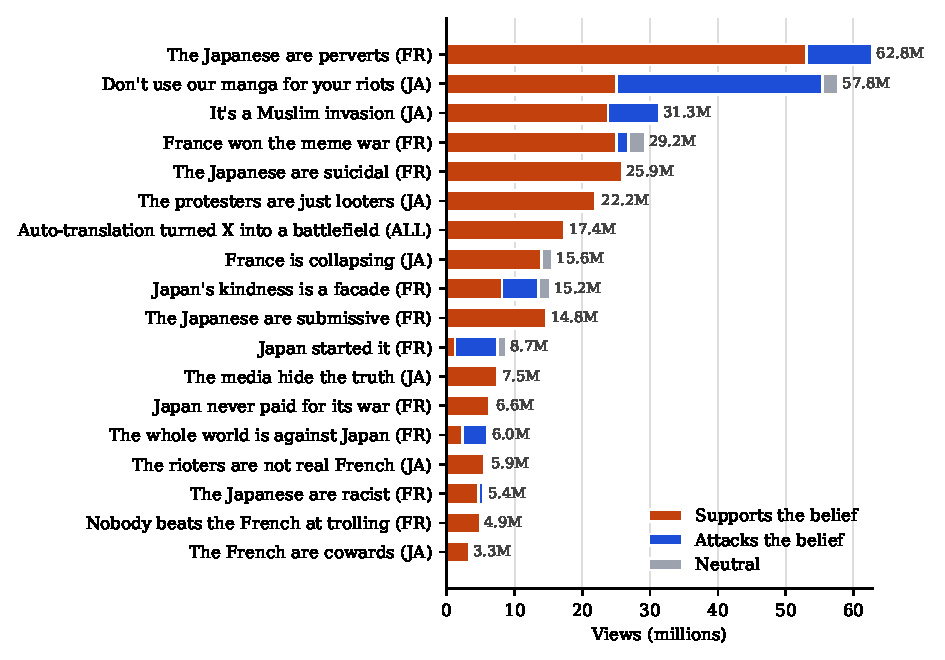
\includegraphics[width=\linewidth]{fig1.pdf}
\caption{Views per belief, split by stance. Owner camp in brackets. No-belief bins excluded. Largest: ``The Japanese are perverts'' (62.8M), ``Don't use our manga for your riots'' (57.8M, of which 30.5M attack it), ``It's a Muslim invasion'' (31.3M).}
\label{fig:beliefs}
\end{figure}

\subsection{In Japan, the riots became an immigration debate}
Four beliefs owned by the Japanese side concern immigration or media distrust: ``It's a Muslim invasion'' (23.8M supporting views), ``France is collapsing'' (13.9M), ``The media hide the truth'' (7.5M) and ``The rioters are not real French'' (5.6M). Together they took 50.8M of 125.5M Japanese-side views (40\%). ``It's a Muslim invasion'' also has the highest Elo of all beliefs (1591; 8 wins, 1 loss across beliefs). Its supporting posts were carried about equally by humor (11.9M) and argument (11.6M).

\subsection{The correction won the duels and lost the reach}
On October 23, Hiroyuki Nishimura, founder of the 2channel forum, posted the Justice Ministry figures in Japanese (2.73M views). Five quote posts answered it in support of the invasion belief; each reached fewer people than his post (5 wins, 0 losses). Overall, inner duels on this belief went 5 to 2 in favor of attackers. Yet posts supporting the belief totaled 23.8M views, 8.7 times the correction. Winning every direct exchange did not translate into reach, consistent with evidence that false news spreads further and faster than true news on Twitter~\cite{vosoughi}.

\subsection{Racism was answered with stereotypes}
The largest French-side beliefs were ``The Japanese are perverts'' (53.1M supporting views), ``The Japanese are suicidal'' (25.9M) and ``The Japanese are submissive'' (14.8M): 93.8M of 193.1M French-side views (49\%). Posts accusing Japan of racism (``The Japanese are racist'') drew 4.7M French-side views (2\%).

\subsection{The manga plea met mockery}
``Don't use our manga for your riots'' drew 25.0M supporting views, all on the Japanese side. Posts attacking it drew 30.5M, mostly French mockery, and won 11 of 12 inner duels. Japanese-speaking critics of the plea added 1.45M views.

\subsection{Packaging}
\begin{table}[h]
\centering\small
\begin{tabular}{lrrr}
\toprule
Register & Posts & Share of posts & Share of views\\
\midrule
Humor & 127 & 39\% & 54\%\\
Argument & 119 & 36\% & 27\%\\
Meta (about the fight itself) & 30 & 9\% & 5\%\\
Insult & 28 & 9\% & 7\%\\
Testimony & 13 & 4\% & 6\%\\
Information & 10 & 3\% & 2\%\\
\bottomrule
\end{tabular}
\caption{Register of the 327 posts. Humor over-performs its share of posts; information under-performs.}
\label{tab:register}
\end{table}
A further 17.4M views went to posts about X's automatic translation itself (``Auto-translation turned X into a battlefield''), a belief shared by all sides. Translation made each camp's posts readable to the other and gave spectators a running joke.

\subsection{Can the beliefs be recovered automatically?}
\begin{table}[h]
\centering\small
\begin{tabular}{llrrr}
\toprule
Input & Encoder & Posts & Ward ARI & $k$-means ARI\\
\midrule
Idea sentence & all-MiniLM-L6-v2 & 327 & 0.14 & 0.15\\
Idea sentence & all-mpnet-base-v2 & 327 & 0.19 & 0.16\\
Raw post text & paraphrase-multilingual-mpnet-base-v2 & 235 & 0.10 & n/a\\
Idea sentence & paraphrase-multilingual-mpnet-base-v2 & 235 & 0.16 & n/a\\
\bottomrule
\end{tabular}
\caption{Unsupervised clustering against the 20 hand labels. ARI 0 is chance, 1 is perfect agreement.}
\label{tab:ari}
\end{table}

\begin{table}[h]
\centering\small
\begin{tabular}{llrrr}
\toprule
Input & Encoder & Posts & Top-1 & Top-3\\
\midrule
Raw post text & multilingual mpnet & 221 & 21.3\% & 46.6\%\\
Idea sentence & multilingual mpnet & 221 & 32.6\% & 58.4\%\\
Idea sentence & multilingual mpnet & 309 & 34.3\% & 59.9\%\\
Idea sentence & all-mpnet-base-v2 & 309 & 33.3\% & 53.4\%\\
\bottomrule
\end{tabular}
\caption{Zero-shot assignment to the 18 belief labels by cosine similarity. Chance: 5.6\%. Majority class: 15.9\% (309 posts).}
\label{tab:zeroshot}
\end{table}

Neither test recovers the beliefs well. Clustering raw posts gives an ARI of 0.10; writing out each post's implied idea raises it to 0.16 with the same multilingual encoder, and to 0.19 with the best English encoder. Zero-shot assignment follows the same pattern: on the same 221 posts, the paraphrase lifts top-1 accuracy from 21.3\% to 32.6\%. The lift holds for humor (26.0\% to 37.5\%, 96 posts) and for argument (16.9\% to 27.3\%, 77 posts). Argument posts score below humor posts on both inputs; one possible reason, untested here, is that arguments about immigration use vocabulary close to several beliefs at once.

\section{Discussion}
Three observations follow. First, the belief, not the joke, is the useful unit: the same invasion belief traveled as memes and as arguments in nearly equal measure, and a meme count would have split it in two. Second, stance matters for reach accounting: the manga belief is the second largest by views, but more than half of those views attack it. Third, duels and reach measure different things. A correction can win every head-to-head exchange and still lose the audience, because supporters of a belief do not need to answer the correction to out-reach it.

For automation, the results point to where the work lies. Sentence encoders compare surface meaning; a meme's belief often sits in what the joke implies, in the image, or in the post it quotes. The paraphrase step, done here by a multimodal model and corrected by a human, carries most of the gain, and even then embedding similarity stays far from the hand labels. A practical pipeline is therefore: collect posts by reach; have a vision-language model write the literal reading and the implied idea; induce belief labels with concept induction~\cite{lloom,topicgpt} and the four-question test; assign belief and stance with a reasoning model rather than nearest-neighbor similarity; and audit a random sample by hand. Stance detection toward a stated target is an established task with shared benchmarks on tweets~\cite{semeval}, which this pipeline can reuse.

\section{Limitations}
The corpus is built from the most viewed posts and from hand-chosen searches; it is not a random sample, and the French side is over-represented among the largest seeds. Views measure reach, not agreement or belief adoption. The first annotation pass was made by an AI assistant; the human author checked the 20 most viewed posts and the belief list, and a human audit of a random sample with agreement statistics is planned for the next version. Quote counts and order in the browser change over time, and deleted or protected posts are missing. The idea sentences were written with the belief list in mind, so the paraphrase scores in Tables~\ref{tab:ari} and~\ref{tab:zeroshot} are an upper bound for that step. Owner camps and default stances are a modeling choice; overrides are listed in the released code.

\section{Contributions and use of AI}
\label{sec:contrib}
This study was run by one human author working with an AI assistant (Claude Opus 5.5, Anthropic) in a single agentic coding session from October 26 to 29, 2026. We report who did what, because the AI assistant did a large share of the reading and annotation.

\emph{Louis Korczowski (author)} set the research question (which ideas carry virality in an attention war, and why) and the project brief. He collected the first seed posts by hand from X search, on both sides, before any automated search, and pointed to posts the pipeline had missed, including the thread that revealed the manga-plea belief. He required that every post be read with its image, flagged off-topic posts that had entered the analysis, and asked for every post to be vetted and re-tagged. He proposed the reframing of concepts as beliefs (``what people believe''), relabeled the first example posts under that framing, and checked the annotations of the 20 most viewed posts (10 per side). He decided the political framing, the display rules, the naming of public figures, and wrote or approved the final text.

\emph{The AI assistant} built the data collection (X API v2 queries, counts, post lookup), ran the language searches (500,000, 250,000 and, for Japanese, 100,000 views) and read the Quotes tabs in a logged-in browser, under the author's supervision. It made the first annotation pass on every post (idea sentence, concept then belief, stance, side, community, register, relation), proposed the first concept list and the four-question belief test, applied the author's corrections, ran the NLP models (sentence embeddings, multidimensional scaling, clustering, zero-shot assignment) and computed all metrics, and drafted the dashboard, the figures and this manuscript.

All interpretation and every claim in this paper are the responsibility of the human author. API usage for the study was capped by the author at 10 USD and stayed under 5 USD.

\section{Ethics and data availability}
No post text is reproduced. Ideas are paraphrased in neutral language. Posts labeled as insults are counted but never linked. Sides are languages and positions, never ethnicity or religion. The only person named is a public figure, for a public post. The belief map, per-post annotations without post text, and code are public: map at \url{https://lkorczowski.github.io/france-vs-japan-X-trend/ideas.html}, repository at \url{https://github.com/lkorczowski/france-vs-japan-X-trend}, method for AI assistants at \url{https://github.com/lkorczowski/content-strategist-AI-cookbook}.

\paragraph{Competing interests.} The author runs STATUR, a viral marketing lab. The study was not commissioned.

\begin{thebibliography}{99}\small
\bibitem{franceinfo} franceinfo. Mobilisation du 17 octobre (live coverage), October 17, 2026. \url{https://www.franceinfo.fr/economie/greve/direct-mobilisation-du-17-octobre-lyceens-etudiants-gilets-jaunes-des-milliers-de-manifestants-attendus-dans-toute-la-france_8241022.html}
\bibitem{wiki} Wikipedia (FR). Manifestations du 17 octobre 2026. Accessed October 28, 2026. \url{https://fr.wikipedia.org/wiki/Manifestations_du_17_octobre_2026}
\bibitem{france24} France 24 / AFP. Violences du 17 octobre : le profil type des personnes \'ecrou\'ees d\'evoil\'e, October 22, 2026. \url{https://www.france24.com/fr/france/20261022-violences-17-octobre-profil-type-personnes-\%C3\%A9crou\%C3\%A9es-d\%C3\%A9voil\%C3\%A9}
\bibitem{nippon} Jiji Press via nippon.com. Permanent residency guidelines revised, October 1, 2026. \url{https://www.nippon.com/en/news/yjj2026100100012/}
\bibitem{mashable} C. Townsend. Why French and Japanese users are beefing on X, explained. Mashable, via Yahoo News, October 26, 2026. \url{https://www.yahoo.com/news/world/articles/why-french-japanese-users-beefing-214654270.html}
\bibitem{vingt} F. Bonassin. Mais pourquoi les Fran\c{c}ais et les Japonais s'embrouillent sur les r\'eseaux sociaux depuis une semaine ? 20 Minutes, October 26, 2026. \url{https://www.20minutes.fr/high-tech/by-the-web/4257599-20261026-pourquoi-francais-japonais-embrouillent-reseaux-sociaux-depuis-semaine}
\bibitem{memecap} E. Hwang, V. Shwartz. MemeCap: A Dataset for Captioning and Interpreting Memes. EMNLP 2023. arXiv:2305.13703.
\bibitem{lloom} M. S. Lam, J. Teoh, J. A. Landay, J. Heer, M. S. Bernstein. Concept Induction: Analyzing Unstructured Text with High-Level Concepts Using LLooM. CHI 2024. arXiv:2404.12259.
\bibitem{topicgpt} C. M. Pham, A. Hoyle, S. Sun, P. Resnik, M. Iyyer. TopicGPT: A Prompt-based Topic Modeling Framework. NAACL 2024. arXiv:2311.01449.
\bibitem{elo} A. E. Elo. The Rating of Chessplayers, Past and Present. Arco, 1978.
\bibitem{sbert} N. Reimers, I. Gurevych. Sentence-BERT: Sentence Embeddings using Siamese BERT-Networks. EMNLP 2019. arXiv:1908.10084.
\bibitem{ldavis} C. Sievert, K. Shirley. LDAvis: A method for visualizing and interpreting topics. Workshop on Interactive Language Learning, Visualization, and Interfaces, ACL 2014.
\bibitem{ari} L. Hubert, P. Arabie. Comparing partitions. Journal of Classification 2:193--218, 1985.
\bibitem{vosoughi} S. Vosoughi, D. Roy, S. Aral. The spread of true and false news online. Science 359(6380):1146--1151, 2018.
\bibitem{semeval} S. Mohammad, S. Kiritchenko, P. Sobhani, X. Zhu, C. Cherry. SemEval-2016 Task 6: Detecting Stance in Tweets. SemEval 2016.
\end{thebibliography}

\end{document}
